\documentclass{report}

\usepackage[margin=1in]{geometry}
\usepackage{graphicx}

\title{Assignment 3\\Network Topological Properties\\[1em]CSCI 479}
\author{Josh Tan}
\date{November 21, 2013}
\setlength\parindent{0pt}

\graphicspath{{Results/}}
\DeclareGraphicsExtensions{.pdf}

\begin{document}
\maketitle

\section*{HcNetwork}

\begin{figure}[htp!]
  \centering
  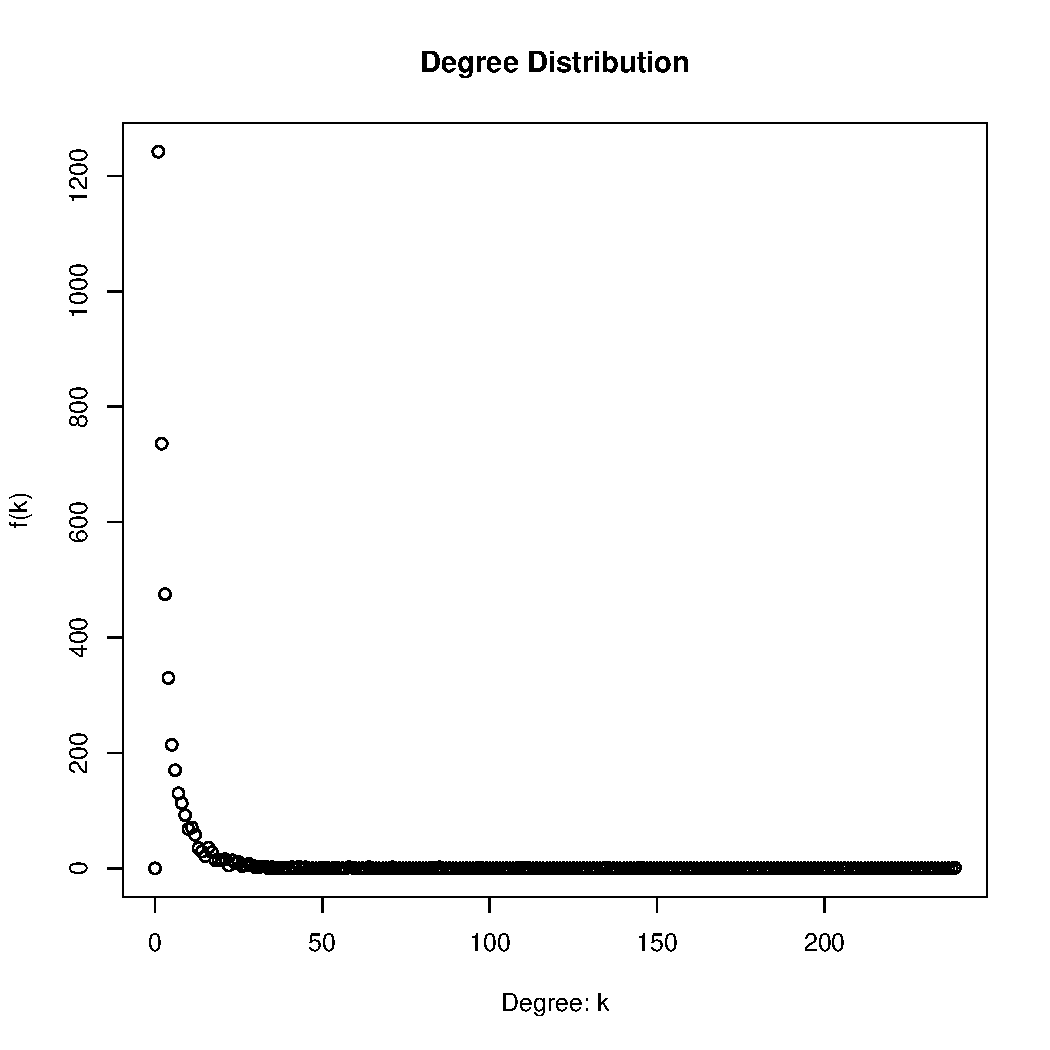
\includegraphics[width=0.65\linewidth]{HcNetwork}
%  \caption{Degree Distribution for HcNetwork network.}
\end{figure}
\vspace{-2em}
\begin{figure}[htp!]
  \centering
  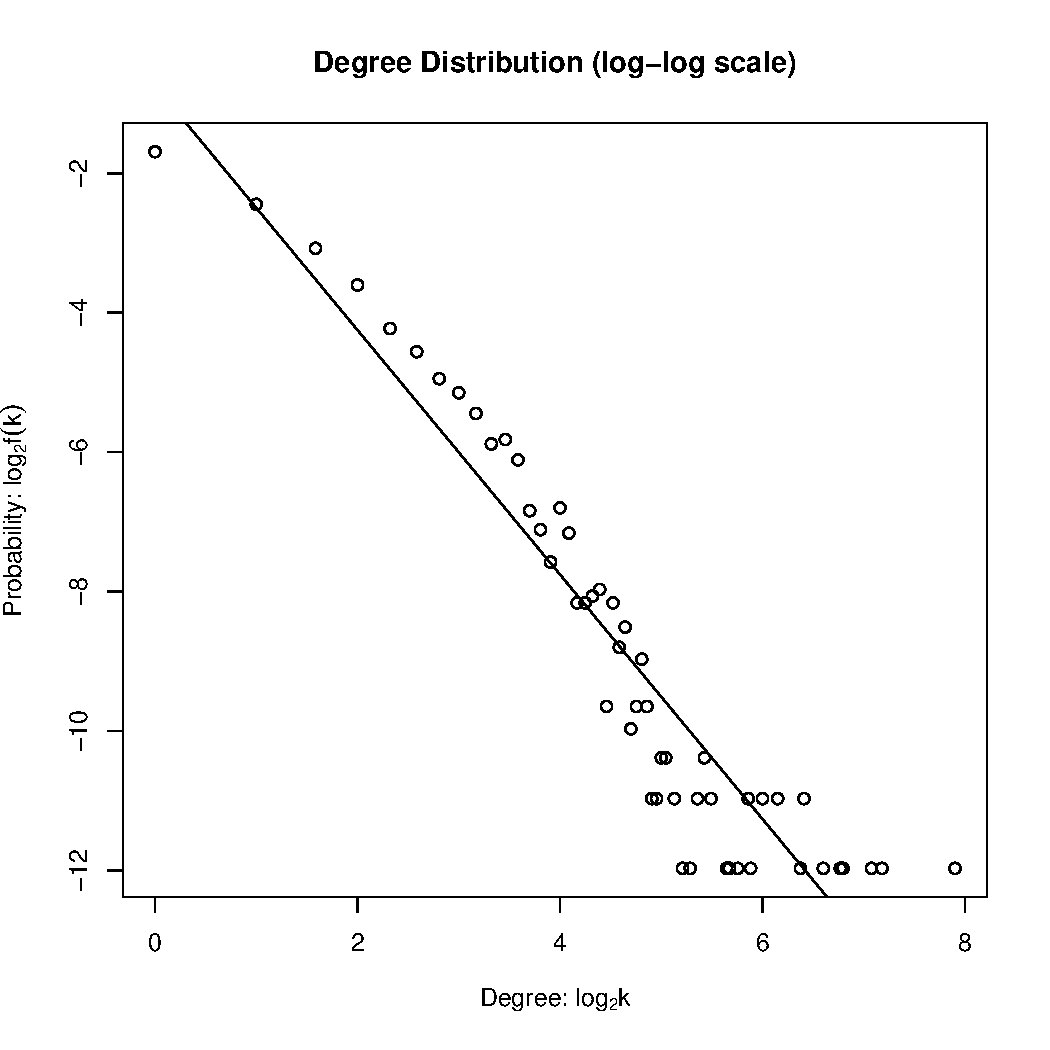
\includegraphics[width=0.65\linewidth]{HcNetworkLog}
%  \caption{Degree distribution probabilities for HcNetwork network, on a log-log scale.}
\end{figure}

\newpage

\section*{HprdNetwork}

\begin{figure}[htp!]
  \centering
  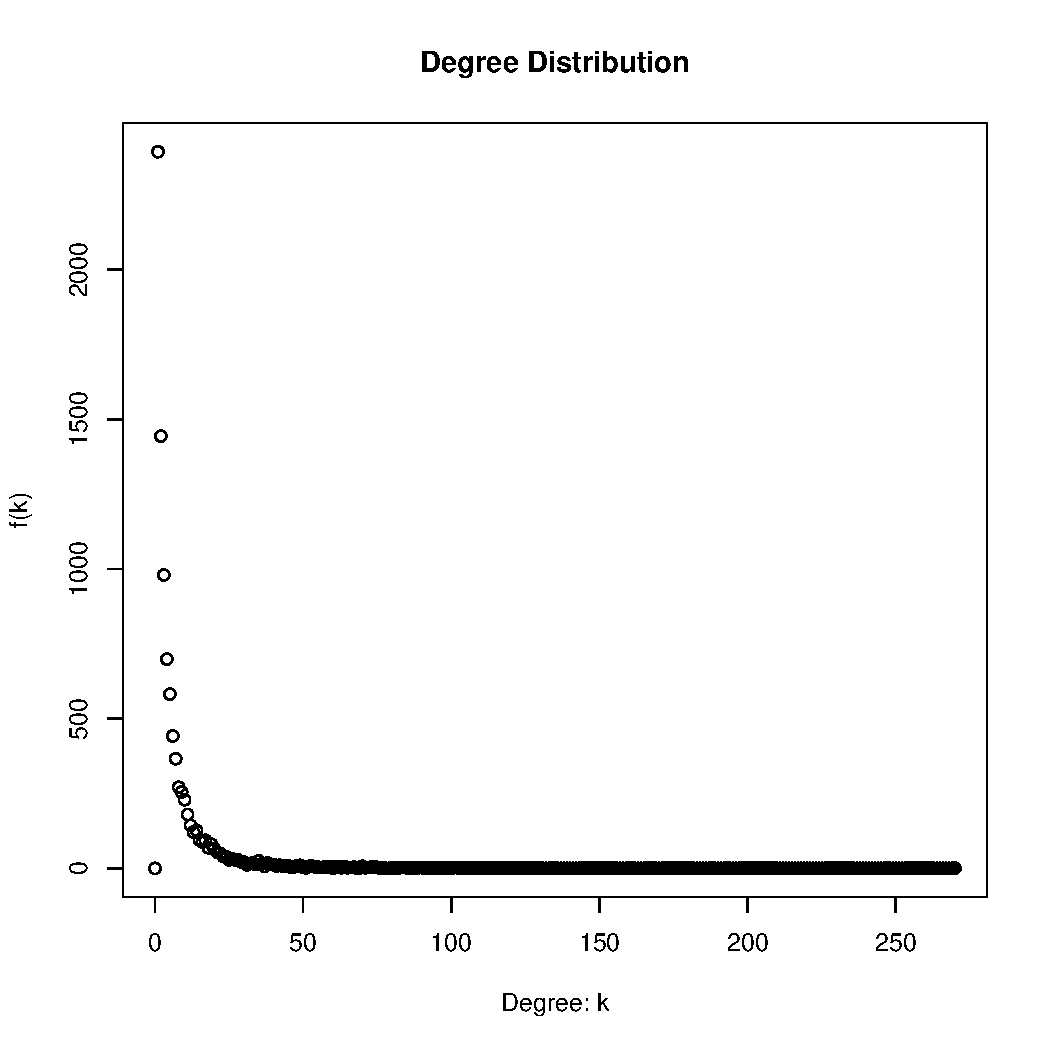
\includegraphics[width=0.65\linewidth]{HprdNetwork}
%  \caption{Degree distribution for HprdNetwork network.}
\end{figure}
\vspace{-2em}
\begin{figure}[htp!]
  \centering
  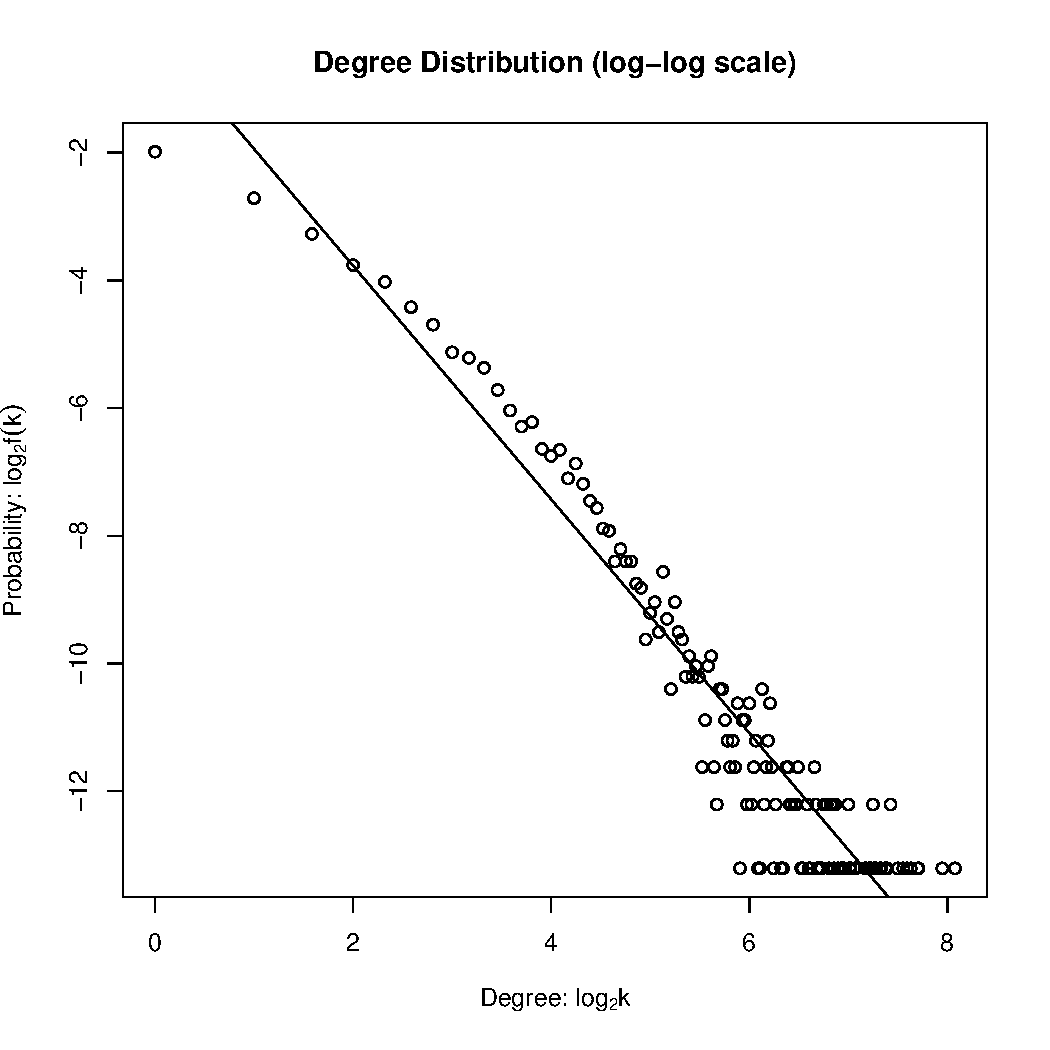
\includegraphics[width=0.65\linewidth]{HprdNetworkLog}
%  \caption{Degree distribution probabilities for HprdNetwork network, on a log-log scale.}
\end{figure}

\newpage

\section*{karate}

\begin{figure}[htp!]
  \centering
  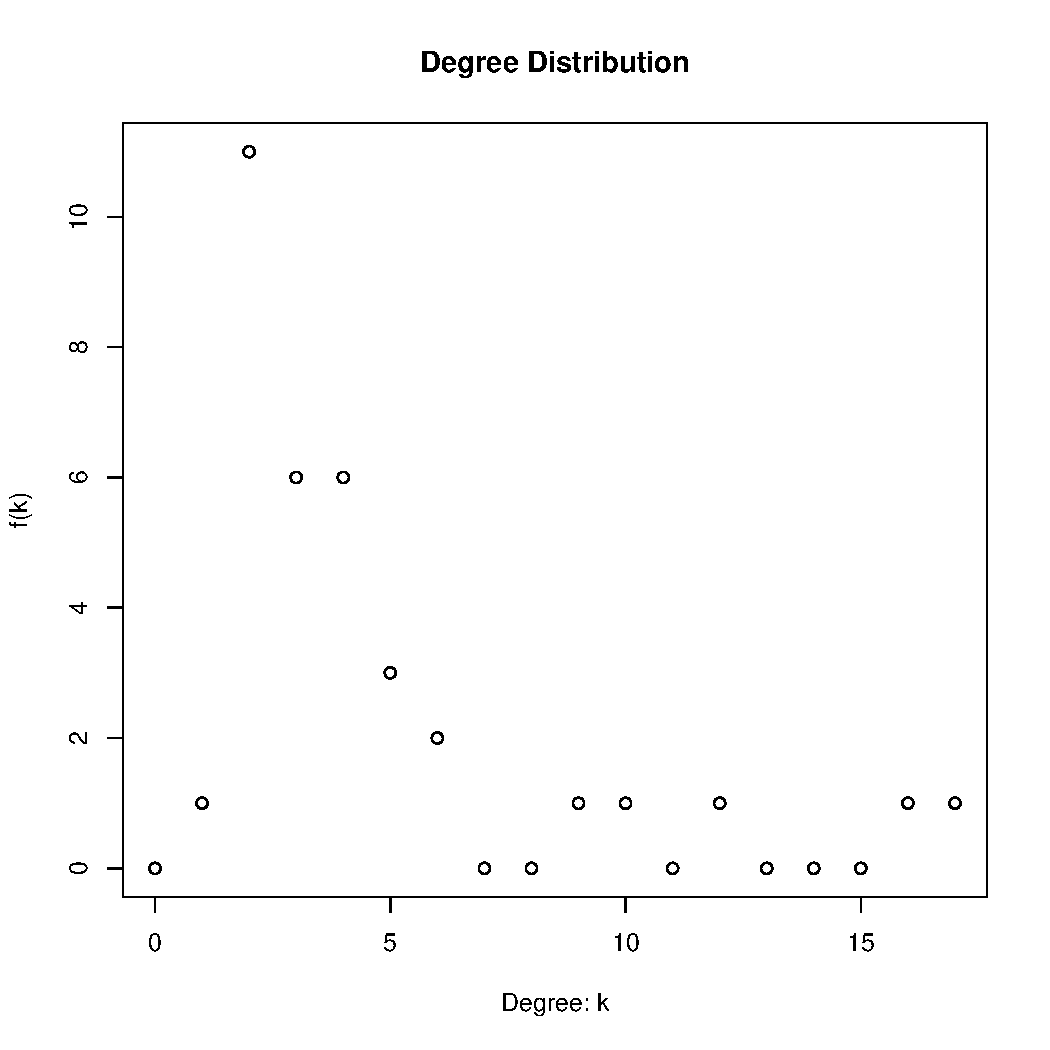
\includegraphics[width=0.65\linewidth]{karate}
%  \caption{Degree distribution for karate network.}
\end{figure}
\vspace{-2em}
\begin{figure}[htp!]
  \centering
  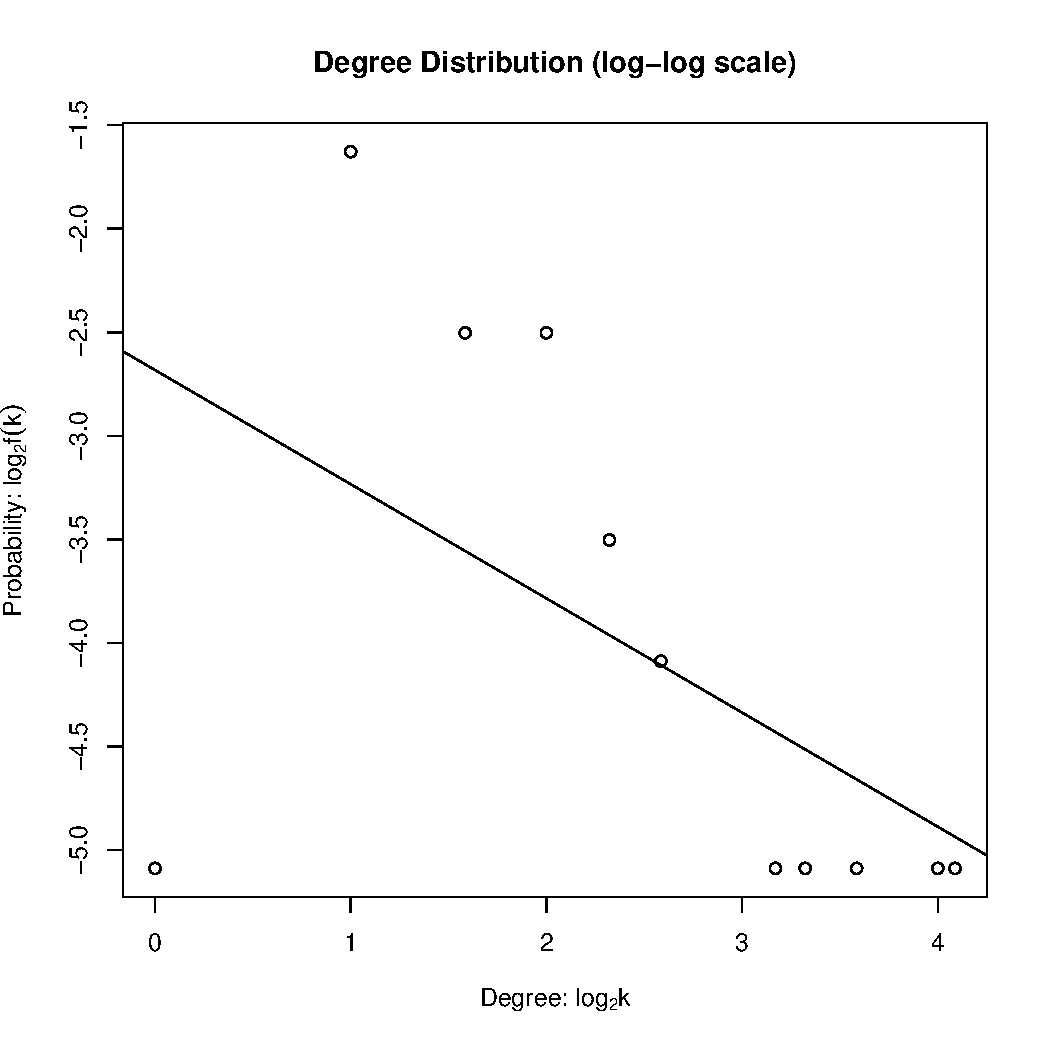
\includegraphics[width=0.65\linewidth]{karateLog}
%  \caption{Degree distribution probabilities for karate network, on a log-log scale.}
\end{figure}

\newpage

\section*{Discussion}

The log-log degree distribution scatter plots for the Yeast and Human protein-protein interaction networks can be fitted a to a linear model fairly well (although there seems to be a high level of noise for the higher degrees). Thus, these two graphs exhibit scale-free behavior.\\

The Karate Club network data, on the other hand, does not allow for a close liner model fitting in the log-log scale, and therefore does not exhibit scale-free behavior.


\end{document}
%%% Local Variables: 
%%% mode: latex
%%% TeX-master: t
%%% End: 
